\documentclass[11pt, 3p]{elsarticle}

\usepackage{lineno}
\modulolinenumbers[5]

\usepackage[short]{optidef}
\usepackage{amsmath}
\usepackage{amssymb}
\usepackage{graphicx}
%\usepackage{subfig}
\usepackage{subcaption,booktabs}
\usepackage{tabularx}
\usepackage{comment}
%\usepackage[hidelinks]{hyperref}
\usepackage{hyperref}
\usepackage{adjustbox}
\usepackage{longtable}
\usepackage{multirow}
\usepackage{multicol}
\usepackage{enumitem}
\usepackage{array}
\usepackage{xcolor}
\usepackage[ruled]{algorithm2e}

\journal{}

\DeclareMathOperator*{\argmax}{arg\,max}
\DeclareMathOperator*{\argmin}{arg\,min}

\newcommand{\bftab}{\fontseries{b}\selectfont}

\newcommand\VP[1]{\textcolor{green}{#1}}
\newcommand\AS[1]{\textcolor{blue}{#1}}
\newcommand\ALC[1]{\textcolor{red}{#1}}

\newtheorem{assumption}{Assumption}
\newtheorem{proposition}{Proposition}

%%% Figures packages and newcommands
\usepackage{tikz}
\usetikzlibrary{arrows.meta, shapes,calc,patterns,decorations.pathmorphing}
\usepackage{pgfplots}
\pgfplotsset{compat=1.16}
\usepackage{subfloat}

%%% TIKZ STYLES
\tikzstyle{none}=[]
\tikzstyle{decision} = [diamond, aspect=2, draw, thick, text width=8em, text badly centered, inner sep=2pt]
\tikzstyle{decision2} = [diamond, aspect=3, draw, thick, text width=17em, text badly centered, inner sep=2pt]
\tikzstyle{block} = [rectangle, draw, thick, text width=17em, text centered, rounded corners, inner sep=5pt]
\tikzstyle{block2} = [rectangle,
    text width=4em, text centered, rounded corners, inner sep=5pt]
\tikzstyle{line} = [draw, thick, -latex]

%%%%%%%%%%%%%%%%%%%%%%%
%% Elsevier bibliography styles
%%%%%%%%%%%%%%%%%%%%%%%
%% Numbered
%\bibliographystyle{model1-num-names}

%% Numbered without titles
%\bibliographystyle{model1a-num-names}

%% Harvard
%\bibliographystyle{model2-names.bst}\biboptions{authoryear}

%% Vancouver numbered
%\usepackage{numcompress}\bibliographystyle{model3-num-names}

%% Vancouver name/year
%\usepackage{numcompress}\bibliographystyle{model4-names}\biboptions{authoryear}

%% APA style
\bibliographystyle{model5-names}\biboptions{authoryear}

%% AMA style
%\usepackage{numcompress}\bibliographystyle{model6-num-names}

%% `Elsevier LaTeX' style
%\bibliographystyle{elsarticle-num}
%%%%%%%%%%%%%%%%%%%%%%%

%\linespread{1.3}
\usepackage{setspace}
\onehalfspacing


\begin{document}

\begin{frontmatter}

%\title{Large-scale Minimum Sum-of-Squares Clustering with Optimality Guarantees}
\title{Strong bounds for large-scale Minimum Sum-of-Squares Clustering}

\author{Anna Livia Croella}
\ead{annalivia.croella@uniroma1.it}
\address{Department of Computer, Control and Management Engineering ''Antonio Ruberti'', \\ Sapienza University of Rome, Via Ariosto 25, 00185, Italy}
\author{Veronica Piccialli\corref{cor1}}
\ead{veronica.piccialli@uniroma1.it}
\address{Department of Computer, Control and Management Engineering ''Antonio Ruberti'', \\ Sapienza University of Rome, Via Ariosto 25, 00185, Italy}
\author{Antonio M. Sudoso}
\ead{antoniomaria.sudoso@uniroma1.it}
\address{Department of Computer, Control and Management Engineering ''Antonio Ruberti'', \\ Sapienza University of Rome, Via Ariosto 25, 00185, Italy}
\cortext[cor1]{Corresponding author}

\begin{abstract}
Clustering is a fundamental technique in data analysis and machine learning, used to group similar data points together. Among various clustering methods, the Minimum Sum-of-Squares Clustering (MSSC) is one of the most widely used. MSSC aims to minimize the total squared Euclidean distance between data points and their corresponding cluster centroids. Due to the unsupervised nature of clustering, achieving global optimality is crucial, yet computationally challenging. The complexity of finding the global solution increases exponentially with the number of data points, making exact methods impractical for large-scale datasets. Even obtaining strong lower bounds on the optimal MSSC objective value is computationally prohibitive, making it difficult to assess the quality of heuristic solutions.
We address this challenge by introducing a novel method to validate heuristic MSSC solutions through optimality gaps. Our approach employs a divide-and-conquer strategy, decomposing the problem into smaller instances that can be handled by an exact solver. The decomposition is guided by an auxiliary optimization problem, the ``anticlustering problem", for which we design an efficient heuristic. Computational experiments demonstrate the effectiveness of the method for large-scale instances, achieving optimality gaps below 3\% in most cases while maintaining reasonable computational times. These results highlight the practicality of our approach in assessing feasible clustering solutions for large datasets, bridging a critical gap in MSSC evaluation.
\end{abstract}

%By leveraging this decomposition, we compute strong lower bounds on the optimal MSSC objective value, enabling the evaluation of optimality gaps for any given feasible clustering solution. 

\begin{keyword}
Machine Learning \sep Minimum sum-of-squares clustering \sep Large scale optimization \sep Clustering validation
\end{keyword}

\end{frontmatter}

\newpage

\section{Introduction}
Clustering is a powerful data analysis tool with applications across various domains. It addresses the problem of identifying homogeneous and well-separated subsets, called \emph{clusters}, from a given set \(O = \{p_1, \ldots, p_N\}\) of \(N\) data observations, each with \(D\) attributes, often referred to as the data dimension \citep{rao1971cluster, hartigan1979algorithm}. Homogeneity means that data within the same cluster should be similar, while separation implies that data observations in different clusters should differ significantly. Clustering is used in fields such as image segmentation, text mining, customer segmentation, and anomaly detection \citep{jain1999data}. % For a more detailed discussion of clustering applications, readers are referred to surveys in [...] and references therein.
The most common type of clustering is partitioning, where we seek a partition \(\mathcal{P} = \{C_1, \ldots, C_K\}\) of \(O\) into \(K\) clusters such that:
\begin{enumerate}
    \item[(i)] \(C_j \neq \emptyset, \quad \forall j=1,\ldots,K\);
    \item[(ii)] \(C_i \cap C_j = \emptyset, \quad \forall i,j=1,\ldots,K\) and \(i \neq j\);
    \item[(iii)] \(\bigcup\limits_{j=1}^{K} C_j = O\).
\end{enumerate}
Clustering methods aim to optimize a given clustering criterion to find the best partition \citep{rao1971cluster}. For that purpose, they explore the exponential solution space of assigning data to clusters.
Let \(\mathcal{P}(O, K)\) denote the set of all \(K\)-partitions of \(O\). Clustering can be viewed as a mathematical optimization problem, where the clustering criterion \(f: \mathcal{P}(O, K) \rightarrow \mathbb{R}\) defines the optimal solution for the clustering problem, expressed as:
\begin{equation} \label{clu_opt}
    \min \ \{f(P): P \in \mathcal{P}(O, K)\}.
\end{equation}
The choice of the criterion \(f\) significantly affects the computational complexity of the clustering problem and is selected based on the specific data mining task. Among many criteria used in cluster analysis, the most intuitive and frequently adopted criterion is the minimum sum-of-squares clustering (MSSC) or $K$-means type clustering \citep{gambella2021optimization}, which is given by
\begin{equation}
    \min \ \sum_{j=1}^K\sum_{i: p_i \in C_{j}} \| p_i - \mu_{j} \|^2,
\end{equation}
where \(\|\cdot\|\) is the Euclidean norm and \(\mu_j\) is the cluster center of the points \(p_i\) in cluster \(C_j\). 

The standard MSSC formulation is a Mixed-Integer Nonlinear Programming (MINLP) problem, which can be expressed as:
\begin{subequations}
\label{eq:MSSCcentroid}
\begin{align}
\textrm{MSSC}(O, K) = \min \ & \sum_{i=1}^N \sum_{j=1}^K \delta_{ij}\left\|p_i - \mu_j\right\|^2  \\
\textrm{s.\,t.} \ & \sum_{j=1}^K \delta_{ij} = 1, \quad \forall i \in [N],\label{eq:MSSCsingle}\\
& \sum_{i=1}^N \delta_{ij} \geq 1, \quad \forall j \in [K],\label{eq:MSSCempty}\\
& \delta_{ij} \in \{0, 1\}, \quad \forall i \in [N], \ \forall j \in [K],\\
& \mu_j \in \mathbb{R}^d, \quad \forall j \in [K],
\end{align}
\end{subequations}
where the notation $[Q]$ with any integer $Q$ denotes the set of indices $\{1,\ldots,Q\}$. The binary decision variable $\delta_{ij}$ expresses whether a data point $i$ is assigned to cluster $j$ ($\delta_{ij}=1)$ or not ($\delta_{ij}=0$). The objective function minimizes the sum of the squared Euclidean distances between the data points and the corresponding cluster centers $\mu_j$. Constraints ~\eqref{eq:MSSCsingle} make sure that each point is assigned to exactly one cluster and constraints ~\eqref{eq:MSSCempty} ensure that there are no empty clusters. Problem \eqref{eq:MSSCcentroid} is a nonconvex MINLP. %since the objective function uses multiplications of the assignment variables $\delta_{ij}$ with the squared norms that depend on the centroids $\mu_j$, which are variables of the problem as well. 
Although not explicitly expressed in the formulation, the centers of the $K$ clusters  $\mu_j$, for $j\in [K]$, are located at the centroids of the clusters due to first-order optimality conditions on the $\mu_j$ variables.

The MSSC is known to be NP-hard in \(\mathbb{R}^2\) for general values of \(K\) \citep{mahajan2012planar} and in higher dimensions even for \(K=2\) \citep{aloise2009complexity}. The one-dimensional case is solvable in polynomial time, with an \(\mathcal{O}(KN^2)\) time and \(\mathcal{O}(KN)\) space dynamic programming algorithm \citep{wang2011ckmeans}. 
Achieving global optimality in MSSC is notoriously challenging in practice. The computational complexity grows exponentially with the number of data points, making exact solutions impractical for large-scale datasets. Consequently, many clustering algorithms resort to heuristic or approximate methods that offer no guarantees about the quality of the solution. However, clustering is a data mining task that requires global optimality. Unlike supervised methods, where class labels are known and a variety of performance measures exist (e.g. precision, recall, F-score), clustering performance and validation are carried out \textit{internally} by optimizing a mathematical function as in~(\ref{clu_opt}) based only on the inter- and intra-cluster relations between the given data observations, or \emph{externally}, by measuring how close a given clustering solution is to a ground-truth solution for a specific data set. However, external validation is limited by the nonexistence of ground-truth solutions, which is why clustering is performed. Since clustering does not rely on side information, its outcome typically requires interpretation by domain experts. Poor-quality heuristic clustering can lead to incorrect interpretations and potentially serious consequences in fields such as medicine and finance.

\newpage

\paragraph{Contributions of our work}
The impossibility of finding global solutions for large-scale instances poses significant challenges in applications where the quality of the clustering directly impacts downstream tasks, such as image segmentation, market segmentation, and bioinformatics. In particular, given the current state-of-the-art solvers, computing exact solutions for MSSC is out of reach beyond a certain instance size. Moreover, for large-scale datasets, even obtaining good lower bounds on the optimal MSSC objective value is prohibitive, making it impossible to assess the quality of heuristic solutions. This work is the first to fill this gap by introducing a method to validate heuristic clustering solutions. Our approach is based on a divide-and-conquer strategy that decomposes the problem into small- and medium-sized instances that can be handled by using exact solvers as a computational engine. Overall, we provide the following contributions:
\begin{itemize}
    \item We propose a scalable procedure to compute strong lower bounds on the optimal MSSC objective value. These bounds can be used to compute an optimality gap for any feasible MSSC solution. The lower bound is obtained by decomposing the original problem into smaller, more tractable subproblems that can either be solved to optimality or provide valid bounds.
    \item The decomposition process is guided by an auxiliary optimization problem, known as the ``anticlustering problem", for which we design an efficient heuristic. Once the decomposition is determined, we leverage optimization again to validate heuristic MSSC solutions through an optimality gap.
    \item The computational results show that the proposed method provides an optimality measure for very large-scale instances. The computed optimality gaps are all below 3\% apart from one instance with gap around 4\%, with many instances exhibiting significantly smaller gaps, while keeping computational times reasonable, below two hours on average.
\end{itemize}

The rest of this paper is organized as follows. Section \ref{sec:lit} reviews the literature related to the MSSC problem, describing heuristics and exact methods. Section \ref{sec:definition}, describes the decomposition strategy and the lower bound computation. Section \ref{sec:avoc} illustrates the algorithm for validating a feasible MSSC solution. Section \ref{sec:results} provides computational results. Finally, Section \ref{sec:conclusions} concludes the paper and discusses research directions for future work.



\section{Literature review} \label{sec:lit}

The most popular heuristic to optimize MSSC is the famous $k$-means algorithm \citep{macqueen1967some, lloyd1982least} ($\approx$ 3M references in Google Scholar 2025). It starts from an initial partition of $O$, so that each data point is assigned to a cluster. In the sequel, the centroids are computed and each point is then assigned to the cluster whose centroid is closest to it. If there are no changes in assignments, the heuristic stops. Otherwise, the
centroids are updated, and the process is repeated. The main drawback of $k$-means is that it often converges to locally optimal solutions that may be far from the global minimum. Moreover, it is highly sensitive to the choice of the initial cluster centers. As a result, considerable research has been devoted to improving initialization strategies (see, e.g.,\cite{arthur2006k,improvedkmeans2018,franti2019much}). 

Several heuristics and metaheuristics have been developed for the MSSC problem. These include simulated annealing \citep{lee2021simulated}, nonsmooth optimization \citep{bagirov2006new, BAGIROV201612}, tabu search \citep{ALSULTAN19951443}, variable neighborhood search \citep{HANSEN2001405,Orlov2018, carrizosa2013variable}, iterated local search \citep{likas2003global}, evolutionary algorithms \citep{MAULIK20001455,SARKAR1997975}), difference of convex functions programming \citep{tao2014new,BAGIROV201612,KARMITSA2017367,KARMITSA2018245}. The \(k\)-means algorithm is also used as a local search subroutine in various algorithms, such as the population-based metaheuristic proposed by \cite{gribel2019hg}.

The methods for solving the MSSC problem to global optimality are generally based on branch-and-bound (B\&B) and column generation (CG) algorithms. The earliest B\&B for the MSSC problem is attributed to \cite{koontz1975branch}, later refined by \cite{diehr1985evaluation}. This method focuses on partial solutions with fixed assignments for a subset of the data points, exploiting the observation that the optimal solution value for the full set is no less than the sum of the optimal solutions for the subsets. \cite{brusco2006repetitive} further developed this approach into the repetitive-branch-and-bound algorithm (RBBA), which solves sequential subproblems with increasing data points. RBBA is effective for synthetic datasets up to 240 points and real-world instances up to 60 data points. Despite being classified as a B\&B algorithm, Brusco's approach does not leverage lower bounds derived from relaxations of the MINLP model. Instead, it relies on bounds derived from the inherent properties of the MSSC problem. In contrast, a more traditional line of research employs B\&B algorithms where lower bounds are obtained through appropriate mathematical programming relaxations of the MINLP model. For example, the B\&B method by \cite{sherali2005global} employs the reformulation-linearization technique to derive lower bounds by transforming the nonlinear problem into a 0-1 mixed-integer program. This method claims to handle problems up to 1000 entities, though replication attempts have shown high computing times for real datasets with around 20 objects \citep{aloise2011evaluating}. More recent efforts by \cite{burgard2023mixed} have focused on mixed-integer programming techniques to improve solver performance, but these have not yet matched the leading exact methods for MSSC.

The first CG algorithm for MSSC problem has been proposed by \cite{du1999interior}. In this algorithm, the restricted master problem is solved using an interior point method while for the auxiliary problem a hyperbolic program with binary variables is used to find a column with negative reduced cost. To accelerate the resolution of the auxiliary problem, variable-neighborhood-search heuristics are used to obtain a good initial solution. Although this approach successfully solved medium-sized benchmark instances, including the popular Iris dataset with 150 entities, the resolution of the auxiliary problem proved to be a bottleneck due to the unconstrained quadratic 0-1 optimization problem. To overcome this issue, \cite{aloise2012improved} proposed an improved CG algorithm that uses a geometric-based approach to solve the auxiliary problem. Specifically, their approach involves solving a certain number of convex quadratic problems to obtain the solution of the auxiliary problem. When the points to be clustered are in the plane, the maximum number of convex problems to solve is polynomially bounded. Otherwise, the algorithm needs to find the cliques in a certain graph induced by the current solution of the master problem to solve the auxiliary problems. The efficiency of this algorithm depends on the sparsity of the graph, which increases as the number of clusters $K$ increases. Therefore, the algorithm proposed by \cite{aloise2012improved} is particularly efficient when the graph is sparse and $K$ is large. Their method was able to provide exact solutions for large-scale problems, including one instance of 2300 entities, but only when the ratio between $N$ and $K$ is small. More recently, \cite{sudoso2024column} combined the CG proposed by \cite{aloise2012improved} with dynamic constraint aggregation \citep{bouarab2017dynamic} to accelerate the resolution of the restricted master problem, which is known to suffer from high degeneracy.  When solving MSSC instances in the plane using branch-and-price, the authors show that this method can handle datasets up to about 6000 data points.

Finally, there is a large branch of literature towards the application of techniques from semidefinite programming (SDP). \cite{peng2005new} and \cite{peng2007approximating} showed the equivalence between the MINPL model and a 0-1 SDP reformulation. \cite{aloise2009branch} developed a branch-and-cut algorithm based on the linear programming (LP) relaxation of the 0-1 SDP model, solving instances up to 202 data points. \cite{piccialli2022sos} further advanced this with a branch-and-cut algorithm using SDP relaxation and polyhedral cuts, capable of solving real-world instances up to 4,000 data points. This algorithm currently represents the state-of-the-art exact solver for MSSC. Additionally, \cite{liberti2022side} examine the application of MINLP techniques to MSSC with side constraints, while the SDP-based exact algorithms proposed in \cite{piccialli2022semi, piccialli2023global} demonstrate state-of-the-art performance for constrained variants of MSSC.



\section{Decomposition strategy and lower bound computation} \label{sec:definition}
By exploiting the Huygens' theorem (e.g., \cite{edwards1965method}), stating that the sum of squared Euclidean distances from individual points to their cluster centroid is equal to the sum of squared pairwise Euclidean distances, divided by the number of points in the cluster, Problem \eqref{eq:MSSCcentroid} can be reformulated as 
\begin{subequations}
\label{eq:MSSC_intdata}
\begin{align}
\textrm{MSSC}(O,K) = \min_{} & \sum_{j=1}^K\frac{\displaystyle\sum_{i=1}^N\sum_{i^\prime=1}^N \delta_{ij}\delta_{i^\prime j}||p_i - p_{i'}||^2 }{\displaystyle\sum_{i=1}^N\delta_{ij}}\\
\text{s.t.}~ & \sum_{j=1}^K \delta_{ij} = 1,\quad \forall i \in [N],\\
& \sum_{i=1}^N \delta_{ij}  \ge 1, \quad \forall j \in [K],\\
& \delta_{ij} \in \{0,1\}, \quad \forall i \in [N], \ \forall j \in [K].
\end{align}
\end{subequations}

%The reformulation derives from the following property of the MSSC objective (exploiting the optimal value of $\mu_j$):
%\[
%\sum_{i=1}^N \sum_{j=1}^K \delta_{ij}\left\|p_i - \mu_j\right\|^2  %= \sum_{i=1}^N \sum_{j=1}^K \delta_{ij}\left\|p_i - \mu_j\pm %\mu\right\|^2  = \sum_{i=1}^N \sum_{j=1}^K \delta_{ij}\left(\|\mu-%\mu_j\|^2+\|p_i-\mu\|^2-2(\mu-\mu_j)^T(p_i-\mu)\right)
%\]
%where $\mu$ is the baricenter of the dataset:
%\[\mu = \frac{\sum_{i=1}^Np_i}{N}.\]
%Then we have
%\[
%\sum_{i=1}^N \sum_{j=1}^K \delta_{ij}\|p_i-\mu\| = \sum_{i=1}^N\|p_i-\mu\|
%\]
%that is constant. Furthermore:

Our idea is to exploit the following fundamental result provided in \cite{koontz1975branch,diehr1985evaluation} and also used in \cite{brusco2006repetitive}. 



\begin{proposition}\label{prop1}\citep{koontz1975branch, diehr1985evaluation}
Assume the dataset $O=\{p_1,\ldots,p_N\}$ is divided into $T$ subsets $\mathcal{S} = \{S_1,\ldots,S_T\}$ such that $\cup_{t=1}^TS_t = O$, $S_t\cap S_{t^\prime}=\emptyset$ and $S_t \neq \emptyset$ for all $t,t^\prime\in [T]$, $t\not=t^\prime$, i.e., $\mathcal{S}$ is a partition of O. 
Assume also that the optimal value of the MSSC problem on each subset is available, i.e., $\textrm{MSSC}(S_t,K)$ is known, for all $t\in [T]$. Then:
\begin{equation}\label{eq:lower}
   \textrm{MSSC}\left(O,K\right)=\displaystyle \textrm{MSSC}\left(\displaystyle\bigcup_{t=1}^T S_t,K\right)   \geq \displaystyle\sum_{t=1}^T \textrm{MSSC}(S_t,K).
\end{equation}
\end{proposition}
Proposition \ref{prop1} states that the sum of the optimal values on all the subsets provides a lower bound on the optimal value of Problem \eqref{eq:MSSCcentroid}.
Moreover, Proposition \ref{prop1}  implies that 
\begin{equation}\label{eq:lower_weak}
   \textrm{MSSC}(O,K)\geq \displaystyle\sum_{t=1}^T  \textrm{MSSC}_\textrm{LB}(S_t,K)
\end{equation}
for any valid lower bound $\textrm{MSSC}_\textrm{LB}(S_t,K)$ of $\textrm{MSSC}(S_t,K)$.


Our idea is to build a partition $\mathcal{S}$ of the dataset $O$ that can be used to compute a tight lower bound on $\textrm{MSSC}(O,K)$, exploiting where possible the ability to solve to global optimality or compute a good lower bound for small-medium-size instances. This approach allows us to validate the quality of a heuristic solution by computing the lower bound \eqref{eq:lower} or \eqref{eq:lower_weak}. Clearly, the quality of the lower bound depends on the partition chosen. Although determining the optimal clustering for each subset can be fast if the subsets are small, smaller subproblems often result in poor bounds (e.g., a subproblem with $K$ observations has an objective value of MSSC equal to zero).

The time required to find and verify the optimal solution is heavily dependent on the quality of the initial subproblems. The ``quality'' here refers to how close the sum of the minimal MSSC for the subproblems is to the minimal MSSC for the complete problem. We argue that one should create subsets that are ``representative'' of the complete dataset, rather than relying on random partitioning into subsets.
Furthermore, the size of the subproblems should allow for efficient computation. Note that a very good lower bound can be found by producing a partition with a small number of sets $T$ where most of the data set is contained in one set, and the other sets contain only a very small number of points.
An extreme case where the lower bound \eqref{eq:lower} provides almost zero optimality gap is if $T=2$, $S_1$ is composed of all points apart from $k$, and $S_2$ contains only the $k$ points closest to the centers of the optimal clusters. However, this partition is useless since computing a valid lower bound on $S_1$ is as difficult as on the original dataset. For this reason, we restrict our attention to the equipartition case, where all the subsets in the partition contain (approximately) the same number of points, and this number is ``tractable''. This ensures that the exact solution can be obtained, or the lower bound \eqref{eq:lower_weak} provides a high-quality approximation within a reduced computational time.
In particular, \textsc{SOS}-\textsc{SDP}, the recent exact solver proposed by \cite{piccialli2022sos}, is able to produce strong and computationally efficient SDP-based bounds within a branch-and-cut algorithm. Moreover, it can solve the root node of the B\&B tree for problems up to 1000 points in a reasonable time, and, in general, provides very good optimality gaps (quite often certifying the global minimum).

To summarise, we restrict ourselves to partitions into subsets of equal size, with the subsets size smaller than 1,000 points, which is the size for which we are able to compute a lower bound efficiently. 
The idea is that if the size of the subsets is comparable, we can efficiently compute all the MSSC single lower bound MSSC$_\textrm{LB}(S_t,K)$. Furthermore, if the quality of the partition is high, the contribution to the overall lower bound of each subset should be comparable and not small. Therefore, the choice of the parameter $T$ is driven by the target size of each subset, which should ensure both tractability of the corresponding MSSC problem and significance of the lower bound contribution.

So, the research question we want to answer is: \textit{Which is the partition $\mathcal{S} = \{S_1, \dots, S_T\}$ of the dataset $O$ into $T$ subsets of equal size maximizing the lower bound obtained by summing up the MSSC objective computed on each subset?}

Therefore, we would like to solve the following problem:
\begin{subequations}
\label{eq:PART}
\begin{align}
\textrm{LB} = \max_{}~ & \sum_{t=1}^T \textrm{MSSC}(S_t,K) \\\label{eq:asspart}
\text{s.t.}~ & \sum_{t=1}^T \xi_{it} = 1,\quad \forall i \in [N],\\\label{eq:cardpart}
& \sum_{i=1}^N \xi_{it}  =  \frac{N}{T}, \quad \forall t \in [T],\\
& \xi_{it} \in \{0,1\}, \quad \forall i \in [N], \ \forall t \in [T],
\end{align}
\end{subequations}
where the binary variables $\xi_{it}$ are equal to 1 if the point $p_i$ is assigned to the subset $S_t$. Constraints \eqref{eq:asspart} require that each point is assigned to a single subset, constraints \eqref{eq:cardpart} require that each subset $S_t$ has a number of elements equal to $N/T$. Note that for simplicity, we assume that $N$ can be divided by $T$. The objective function is the solution of the following problem:
\begin{subequations}
\label{eq:MSSC}
\begin{align}
\textrm{MSSC}(S_t, K) = \min_{} & \sum_{j=1}^K \frac{\sum_{i=1}^N  \sum_{i'=1}^N \delta^t_{ij} \delta^t_{i'j} ||p_i - p_{i'}||^2 }{\sum_{i=1}^N \delta^t_{ij}}\\\label{eq:connect}
\text{s.t.}~ & \sum_{j=1}^K \delta^t_{ij} = \xi_{it},\quad \forall i \in [N],\\
& \sum_{i=1}^N \delta^t_{ij}  \ge 1, \quad \forall j \in [K],\\
& \delta^t_{ij} \in \{0,1\}, \quad \forall i \in [N], \ \forall j \in [K]\; %\forall t \in [T].
\end{align}
\end{subequations}
that is the MSSC problem on each subset $S_t$. The two problems are linked by constraints \eqref{eq:connect}, which impose that the data points assigned to the subset $S_t$ must be assigned to the $K$ clusters.


However, Problem \eqref{eq:PART} is not directly solvable, due to its bilevel nature. This undesirable bilevel nature could be avoided if the optimal clustering for any subset was known in advance and independent of the chosen partition. In this case, the optimization variables of the second level would be known, and the problem would become a single-level one.

This occurs for example if the optimal cluster assignment does not change when the MSSC is solved on the single subset $S_t$. In particular, we define   the ``projection'' of the solution $\delta_{ij}$ on the partition $\mathcal{S} = \{S_1, \ldots, S_T\}$ as:
\[
\Delta(\mathcal{S},\delta) =  \left\{\delta_{ij}^t\, : \forall i \in [N], \, \forall j \in [K], \, \forall t\in [T] \right\},
\]
where the clustering assignment $\delta$ is mapped on each subset $S_t$ as follows:
\[
\delta_{ij}^t = 
\begin{cases}
    \begin{array}{lr}
    \delta_{ij}, & \forall i:p_i\in S_t, \ \forall j \in [K], \ \forall t\in [T],\\
    0, & \forall i:p_i\not\in S_t, \ \forall j \in [K], \ \forall t\in [T].
    \end{array}
\end{cases}
\]
From now on we suppose the following assumption to be verified:
\begin{assumption} \label{ass1}
    Let $\delta^*$  be a feasible (possibly optimal) solution of the original MSSC problem. Then for any partition ${\cal S} = \{S_1, \ldots, S_T\}$ of the dataset, the projection $\Delta(\mathcal{S},\delta^*)$ is optimal, that is, $\Delta(\mathcal{S},\delta^*)$ solves MSSC$(S_t, K)$ for all $t\in [T]$. 
\end{assumption}

Assumption \ref{ass1} implies that the optimal solution of the MSSC($S_t$,$K$) is  $\delta^*$ restricted to $S_t$ for all $t\in [T]$.
Given the solution $\delta^*$, we can derive the corresponding clusters $C_j$ for every $j\in [K]$.
In the following, w.l.o.g., we assume that the number of points in each cluster $C_j$, for $j \in [K]$, is a multiple of $T$; that is, $|C_j|/T \in \mathbb{Z}$.
Under Assumption \ref{ass1}, Problem \eqref{eq:PART} can be written as follows:

\begin{subequations}
\label{eq:lui}
\begin{align}
\textrm{LB} = \max_{} &  \sum_{t=1}^{T} \sum_{j=1}^K \sum_{i: p_i\in C_j} \sum_{i': p_{i'} \in C_j} \frac{\|p_i-p_{i'}\|^2}{|C_j|/T} \cdot \xi_{it} \cdot \xi_{i't}  \\
\text{s.t.}~ & \sum_{t=1}^T \xi_{it} = 1,\quad \forall i \in [N],\\
& \sum_{i:p_i\in C_j} \xi_{it} =  \frac{|C_j|}{T}, \quad \forall t \in [T], \ \forall j \in [K],\\
& \xi_{it} \in \{0,1\}, \quad \forall i \in [N], \ \forall t \in [T].
\end{align}
\end{subequations}
Problem \eqref{eq:lui} can be decomposed in $K$ independent subproblems, one for each cluster $C_j$ with $j \in [K]$:
\begin{subequations}
\label{eq:cls}
\begin{align}
\max_{} &  \sum_{t=1}^{T} \sum_{i: p_i\in C_j} \sum_{i': p_{i'} \in C_j} \frac{\|p_i-p_{i'}\|^2}{|C_j|/T} \cdot \xi_{it} \cdot \xi_{i't}\\
\text{s.t.}~ & \sum_{t=1}^T \xi_{it} = 1,\quad \forall i:p_i \in C_j,\\
& \sum_{i: p_i \in C_j} \xi_{it} =  \frac{|C_j|}{T}, \quad \forall t \in [T],\\
& \xi_{it} \in \{0,1\}, \quad \forall i \in C_j\; \forall t \in [T].
\end{align}
\end{subequations}
Problem \eqref{eq:cls} is related to the so-called ``anticlustering problem'', first defined in \cite{spath1986anticlustering}. The goal is to partition a set of objects into groups with high intragroup dissimilarity and low intergroup dissimilarity, meaning that the objects within a group should be as diverse as possible, whereas pairs of groups should be very similar in composition.  In \cite{spath1986anticlustering}, the objective was to maximize rather than minimize the within-group sum-of-squares criterion, which translates into Problem \eqref{eq:cls}. 
The term ``anticlustering'' is used in psychological research, where many applications require a pool of elements to be partitioned into multiple parts while ensuring
that all parts are as similar as possible.  As an example, when dividing students into groups in a school setting, teachers are often interested in assembling groups that are
similar in terms of scholastic ability and demographic composition. In educational
psychology, it is sometimes necessary to divide a set of test items into parts of equal length that are presented to different cohorts of students. To ensure fairness of the test, it is required that all parts be equally difficult. 

The anticlustering problem is also considered in
\cite{papenberg2021using,brusco2020combining,papenberg2024k}, where different diversity criteria and heuristic algorithms are proposed. Problem \eqref{eq:cls} can also be related to the Maximally Diverse Grouping Problem (MDGP) \citep{LAI2016780,schulz2023balanced,schulz2023balanceda,SCHULZ202142}, where the set of vertices of a graph has to be partitioned into disjoint subsets of sizes within a given interval, while maximizing the sum of the edge weights in the subset. In this context, the weights represent the distances between the nodes. MDGP belongs to the category of vertex-capacitated clustering problems
\citep{johnson1993min}.
From now on, we call \textit{anticlusters} the subsets $S_t$ for $t\in[T]$.


Note that even if Assumption \ref{ass1} holds, the anticlustering partition can significantly influence the quality of the lower bound. As an example, in Figure \ref{fig:exdataA} we report a synthetic dataset of 64 points with 4 naturally well-separated clusters (see Figure \ref{fig:exdataB}), which satisfies Assumption \ref{ass1}. In Figures \ref{fig:example} and \ref{fig:example2} we report two different partitions in 4 anticlusters starting from the optimal solution reported in Figure \ref{fig:exdataB}. The first anticluster partition in Figure \ref{fig:example} provides an optimality gap of 32\%, where we can see that the anticluster partition reported in Figure \ref{fig:example2} provides an optimality gap of 0\% certifying the global optimality of the solution. The second partition represents the original dataset better than the first one: in each anticluster, the cluster centroids are very close to the cluster centroids of the starting solution, and the points are far away from each other, showing high dissimilarity.

This simple example shows the need to carefully choose the anticluster partition by solving Problem \eqref{eq:cls}. However, Problem \eqref{eq:cls} can be solved exactly only for very small size instances, therefore, we define an \textit{ad hoc} heuristic for the problem. Note that if Assumption \ref{ass1} does not hold, the lower bound estimate found by solving problems \eqref{eq:cls} and summing up the objective values may be different from the one found by actually solving each MSSC($S_t$, $k$). However, the latter is still valid for MSSC($O$, $k$).


\begin{figure}[!ht]
    \centering
    \begin{subfigure}{0.45\textwidth}
        \includegraphics[scale=0.45]{Figures/data.png}
        \caption{A synthetic dataset of $N=64$ data points with $K=4$ natural well-separated clusters.}
        \label{fig:exdataA}
    \end{subfigure}
    \begin{subfigure}{0.45\textwidth}
        \includegraphics[scale=0.45]{Figures/solw_p.png}
        \caption{Optimal clustering partition for $K=4$ cluster for the synthetic dataset in Figure (a).}
        \label{fig:exdataB}
    \end{subfigure}
    \caption{A synthetic dataset of $N=64$ points with $K=4$ natural well-separated clusters and its optimal clustering partition.}
    \label{fig:exdata}
\end{figure}



\begin{figure}[!ht]
    \centering
    \begin{subfigure}{0.45\textwidth}
        \caption{MSSC$_\textrm{LB}(S_1, 4)= 25.715$}
        \includegraphics[scale=0.45]{Figures/solw_p1.png}
        \label{fig:sol1w}
    \end{subfigure}
    \begin{subfigure}{0.45\textwidth}
        \caption{MSSC$_\textrm{LB}(S_2, 4)= 25.715$}
        \includegraphics[scale=0.45]{Figures/solw_p2.png}
        \label{fig:sol2w}
    \end{subfigure}\\
    \hspace{-1.3cm}
    \begin{subfigure}{0.45\textwidth}
        \centering
        \caption{MSSC$_\textrm{LB}(S_3, 4)= 25.715$}
        \includegraphics[scale=0.45]{Figures/solw_p3.png}
        \label{fig:sol3w}
    \end{subfigure}
    \begin{subfigure}{0.45\textwidth}
        \centering
        \caption{MSSC$_\textrm{LB}(S_4, 4)= 25.715$}
        \includegraphics[scale=0.45]{Figures/solw_p4.png}
        \label{fig:sol4w}
    \end{subfigure}
    \caption{A clustering partition for a dataset of $N = 64$ points, with $K = 4$ clusters and $T=4$ anticlusters. The $UB = MSCC(O,K) =  575.673$ and MSSC$_\textrm{LB}(\mathcal{S}, K) = LB^+ = 102.86$ and $\gamma_\textrm{\tiny LB} = \gamma^+ = 0.82$}
    \label{fig:example}
\end{figure}

\begin{figure}[!ht]
    \centering
    \begin{subfigure}{0.45\textwidth}
        \caption{MSSC$_\textrm{LB}(S_1, 4)= 144.000$}
        \includegraphics[scale=0.45]{Figures/sol_p1.png}
        \label{fig:sol1}
    \end{subfigure}
    \begin{subfigure}{0.45\textwidth}
        \caption{MSSC$_\textrm{LB}(S_2, 4)= 143.926$}
        \includegraphics[scale=0.45]{Figures/sol_p2.png}
        \label{fig:sol2}
    \end{subfigure}\\
    \hspace{-1.3cm}
    \begin{subfigure}{0.45\textwidth}
        \centering
        \caption{MSSC$_\textrm{LB}(S_3, 4)= 143.821$}
        \includegraphics[scale=0.45]{Figures/sol_p3.png}
        \label{fig:sol3}
    \end{subfigure}
    \begin{subfigure}{0.45\textwidth}
        \centering
        \caption{MSSC$_\textrm{LB}(S_4, 4)= 143.926$}
        \includegraphics[scale=0.45]{Figures/sol_p4.png}
        \label{fig:sol4}
    \end{subfigure}
    \caption{Optimal clustering partition for a dataset of $N = 64$ points, with $K = 4$ clusters and $T=4$ anticlusters. The $UB = MSCC(O,K) =  575.673$ and MSSC$_\textrm{LB}(\mathcal{S}, K) = LB^+ = $ and $\gamma_\textrm{\tiny LB} = \gamma^+ = 0.00$}
    \label{fig:example2}
\end{figure}


\section{AVOC: Anticlustering Validation Of Clustering}  \label{sec:avoc}

We propose a heuristic algorithm, named Anticlustering Validation Of Clustering (\textsc{AVOC}), that validates a given clustering partition $\mathcal{P} = \{C_1, \ldots, C_K\}$ of the clustering problem with $K$ clusters on a set of points $O$ with objective function value $UB$.
The algorithm is based on the iterative refinement of an initial anticlustering partition $\mathcal{S} = \{S_1, \dots, S_T\}$ through a swap procedure that aims to maximize the objective of Problem \eqref{eq:lui}.
Specifically, the algorithm includes the following key components: (i) an initialization procedure to produce a feasible anticlustering partition; (ii) an evaluation mechanism that produces an approximation $LB^+$ for the value $LB$; (iii) a heuristic mechanism that iteratively refines the current anticlustering partition to improve the value of $LB^+$; (iv) an algorithm that, given an anticlustering partition, produces a lower bound on the value $\textrm{MSSC}(O,K)$. A schematic representation of the \textsc{AVOC} algorithm is given in Figure \ref{fig:flow}. The pseudocode is outlined in Algorithm 1.

\begin{figure}[]
    \centering
    \scalebox{0.65}{    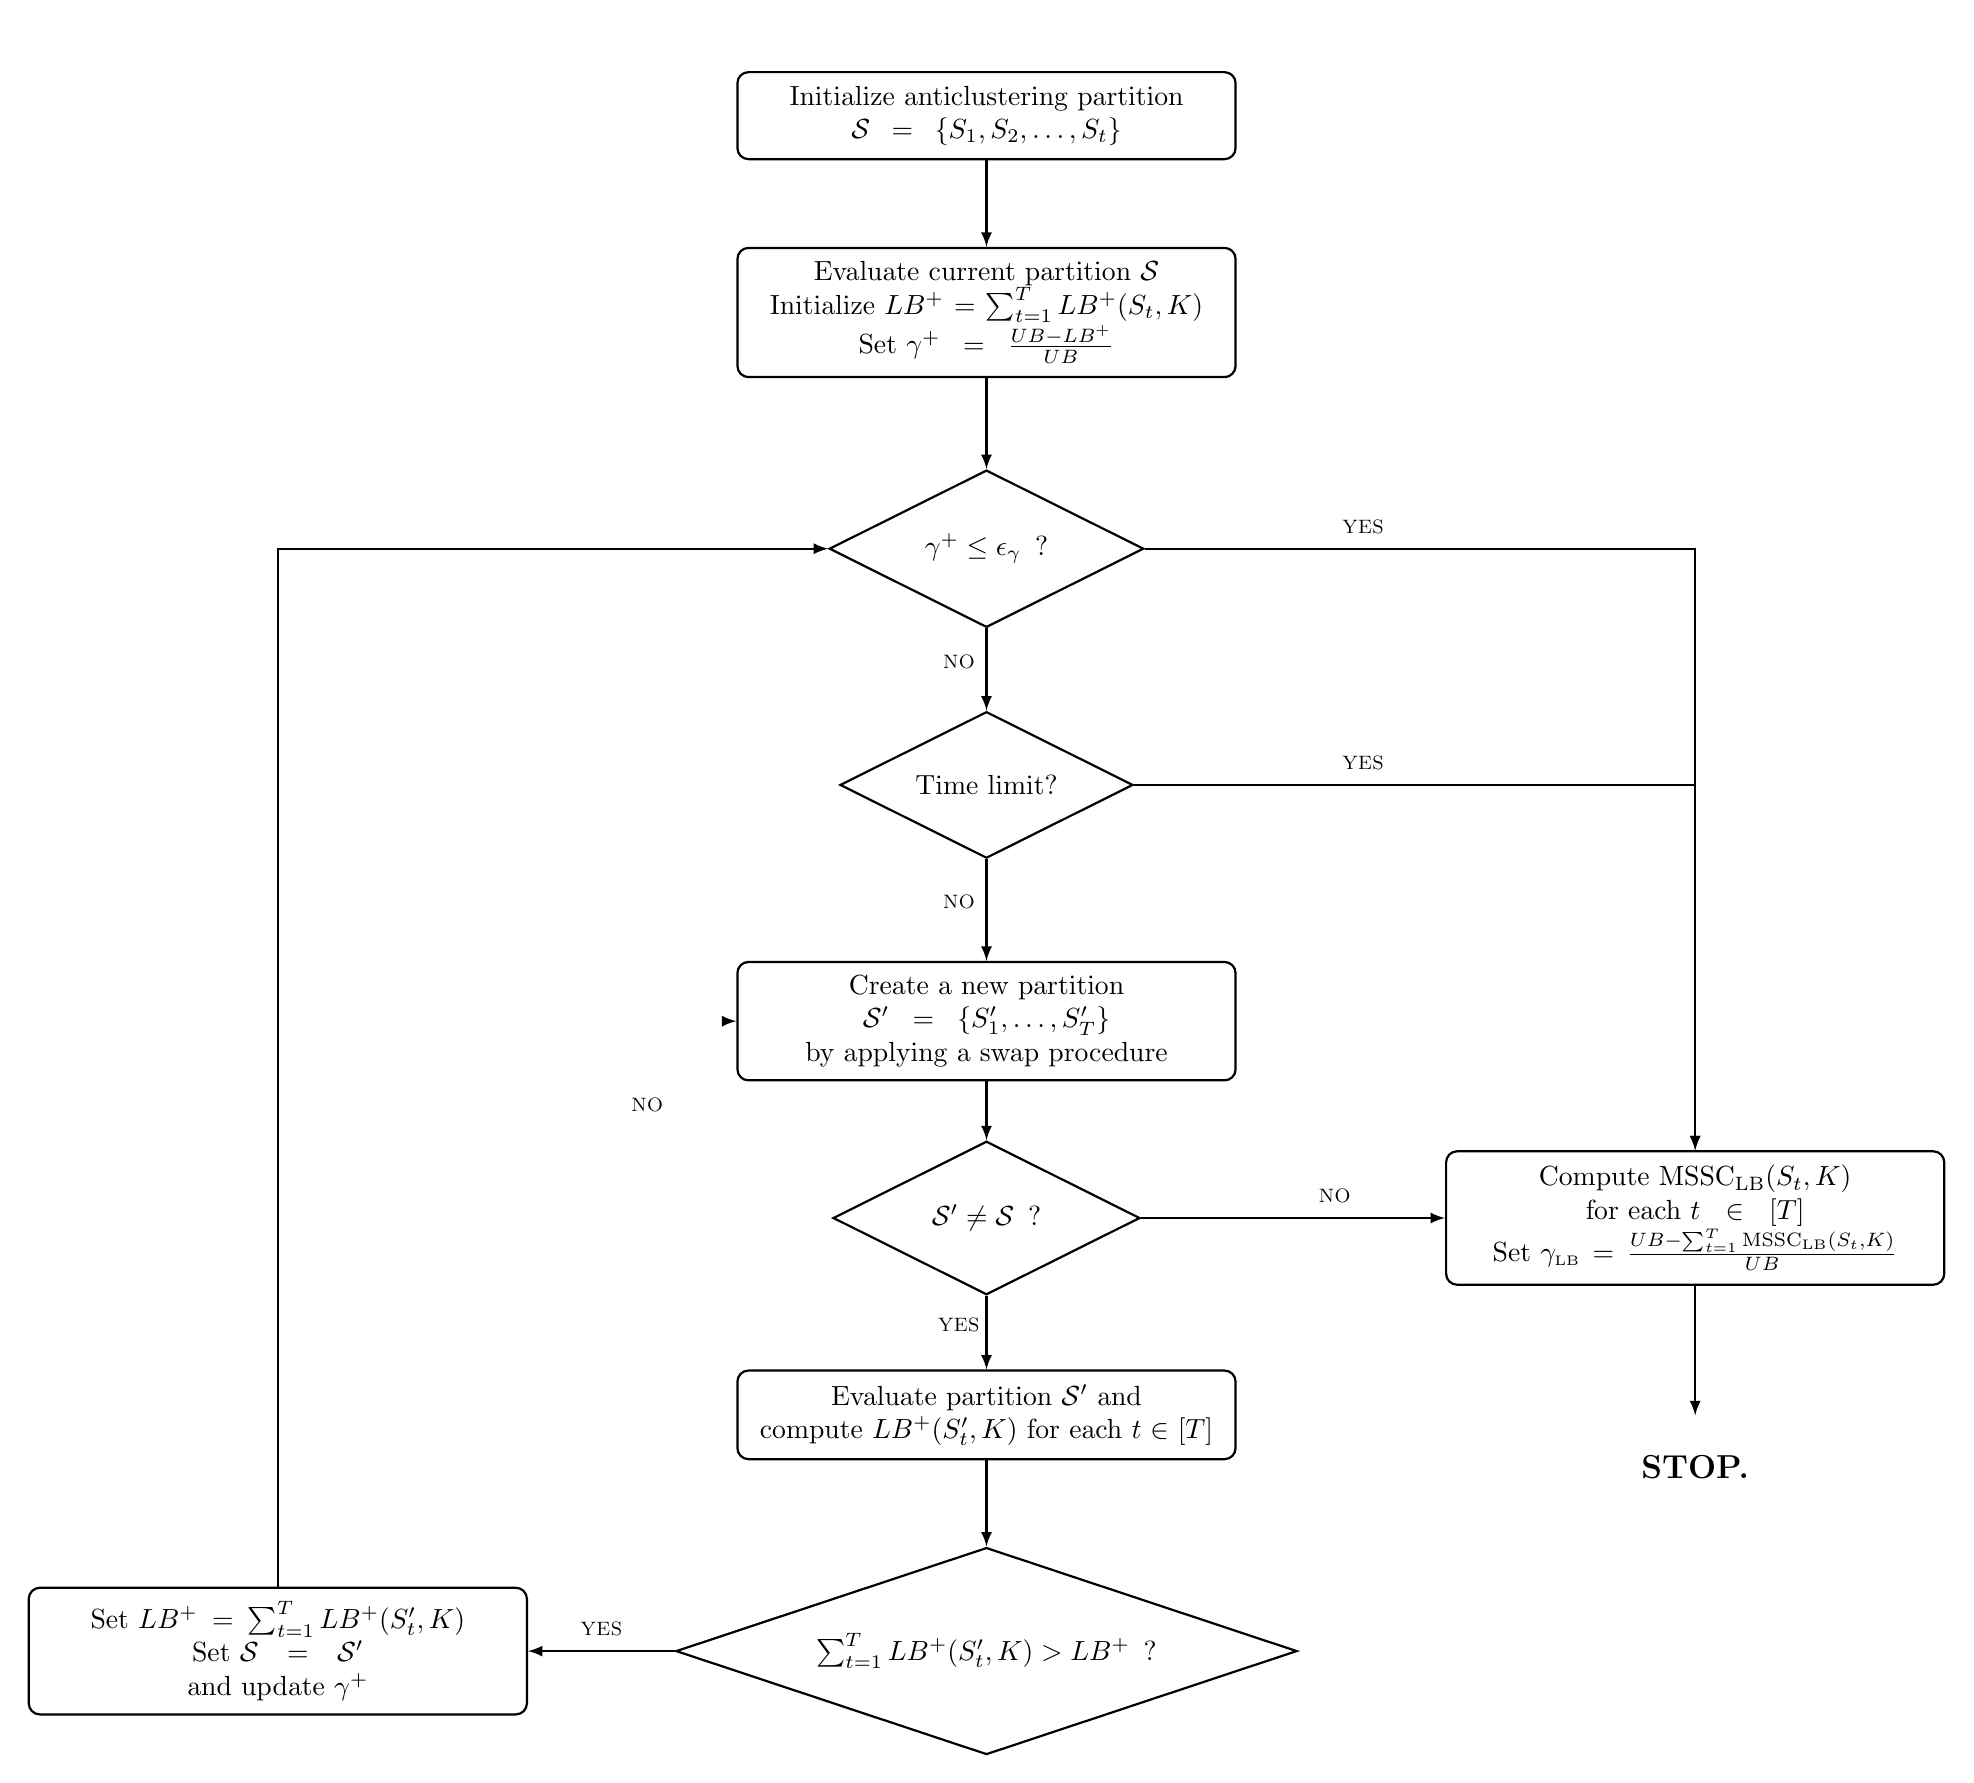
\begin{tikzpicture}[scale=0.5]

        \node [block] (init) {Initialize anticlustering partition\\
        $\mathcal{S} = \{S_1, S_2, \ldots, S_t\}$};

        %\node [cylinder, aspect=.5, minimum height=7mm, cylinder uses custom fill, cylinder body fill=blue!30, draw, left of=init, node distance=9cm] (data) {$O, \, K,\, \mathcal{P}, \, UB$};

        %\node[left of=init, node distance=9cm] (img) {\includegraphics[width=1.8cm]{Figures/avoc.png}};
    
        \node [block, below of=init, node distance=2.5cm] (find) {Evaluate current partition $\mathcal{S}$\\
        Initialize $LB^+ = \sum_{t = 1}^{T} LB^+(S_t,K)$\\
        Set $\gamma^+ = \frac{ UB - LB^+}{UB}$};
        
        \node [decision, below of=find, node distance=3cm] (evaluate) {$\gamma^+ \leq \epsilon_{\gamma}$\, ?};
                
        \node [decision, below of=evaluate, node distance=3cm] (time) {Time limit?};
                
        \node [block, below of=time, node distance=3cm] (ubsol) {Create a new partition $\mathcal{S}' = \{S'_1, \ldots, S'_T\}$\\ by applying a swap procedure};
                
        \node [decision, below of=ubsol, node distance=2.5cm] (improv) {$\mathcal{S}' \neq \mathcal{S}$\, ?};
        
        \node [block, below of=improv, node distance=2.5cm] (differs) {Evaluate partition $\mathcal{S}'$
        and\\ compute $LB^+(S'_t,K)$ for each $t\in [T]$};
        
        \node [decision2, below of=differs, node distance=3cm] (update) {$\sum_{t = 1}^{T} LB^+(S'_t,K) > LB^+$\, ?};
        
        \node [block, left of=update, node distance=9cm] (evaluate2) {
        Set $LB^+ = \sum_{t = 1}^{T} LB^+(S'_t,K)$\\
        Set $\mathcal{S}=\mathcal{S}'$\\
        and update $\gamma^+$\\};
        
        \node [block, right of=improv, node distance=9cm] (compute) {Compute MSSC$_\textrm{LB}(S_t, K)$ for each $t\in[T]$\\
        Set $\gamma_\textrm{\tiny LB} = \frac{UB - \sum_{t=1}^T \textrm{MSSC}_\textrm{LB}(S_t, K)}{UB}$
        };
        
        \node [block2, below of=compute, node distance=3cm] (stop) {\vspace{0.2cm} \large \textbf{\textsc{STOP.}}};
        
        \path [line] (init) -- (find);
        \path [line] (find) -- (evaluate);
        \path [line] (evaluate) -- node[label=\textsc{\scriptsize NO}, yshift=-0.7em, xshift=-1em] {} (time);
        \path [line] (time) -- node[label=\textsc{\scriptsize NO}, yshift=-0.7em, xshift=-1em] {} (ubsol);
        \path [line] (time) -| node[label=\textsc{\scriptsize YES}, yshift=-0.2em, xshift=-12em] {} (compute);
        \path [line] (ubsol) -- (improv);
        \path [line] (improv) -- node[label=\textsc{\scriptsize YES}, yshift=-0.7em, xshift=-1em] {} (differs);
        \path [line] (differs) -- (update);
        \path [line] (update) -- node[label=\textsc{\scriptsize YES}, yshift=-0.2em, xshift=0em] {} (evaluate2);
        \path [line] -- ($(update.west)$) |- node[label=\textsc{\scriptsize NO}, yshift=-4em, xshift=-1em] {} (ubsol);
        \path [line] (evaluate2) |- (evaluate);
        \path [line] (improv) -- node[label=\textsc{\scriptsize NO}, yshift=-0.2em, xshift=1.5em] {} (compute);
        \path [line] (evaluate) -| node[label=\textsc{\scriptsize YES}, yshift=-0.2em, xshift=-12em] {} (compute);
        \path [line] (compute) -- (stop);
        
        % \node[below of=stop]{};
        \node[right of=find, node distance=4cm]{};
        \node[above of=init]{};
        
    \end{tikzpicture}}
    \caption{Flowchart of the \textsc{AVOC} algorithm.}
    \label{fig:flow}
\end{figure}


\subsection{Initialize the \textsc{AVOC} algorithm}

Given a clustering partition $\mathcal{P}$, we generate an initial anticlustering partition $\mathcal{S} = \{S_1, \dots, S_T\}$. The process begins by randomly distributing an equal number of points from each cluster $j \in [K]$, that is $|C_j|/T$ points, into subsets $S_{jt}$ for $t \in [T]$. These subsets are then combined to form an initial anticlustering partition $\mathcal{S}$. To ensure feasibility, each anticluster $S_t$ must include exactly one subset from each cluster.
If Assumption \ref{ass1} holds, all possible combinations of the subset will lead to the same lower bound value. However, if Assumption \ref{ass1} does not hold, different combinations of subsets can affect the quality of the resulting $LB^+$ and hence of $LB$. For this reason, a mixed-integer linear programming (MILP) model is used to determine the optimal combination. The model reads as follows:
\begin{subequations}
\label{eq:mount}
\begin{align}
\label{obj} \max & \sum_{t=1}^{T} \sum_{m=1}^{T} \sum_{m'=m}^{T} \sum_{j=1}^{K} \sum_{j'=j+1}^{K} d_{jj'mm'} \, y^{t}_{jj'mm'}  \\
\label{c:one} \text{s.t.}~ & \sum_{t=1}^T x_{jm}^{t} = 1,\quad \forall j \in [K], \, \forall m \in [T],\\
\label{c:two} & \sum_{m=1}^T x_{jm}^{t} = 1,\quad \forall j \in [K], \, \forall t \in [T],\\
\label{c:three} & y^{t}_{jj'mm'} \leq x_{jm}^{t}, \quad \forall j, j' \in [K], \, \, j<j', \ \forall m,m',t \in [T], \ m \leq m',\\
& y^{t}_{jj'mm'} \leq x_{j'm'}^{t}, \quad \forall j, j' \in [K], \ j<j', \ \forall m,m',t \in [T], \ m \leq m',\\
\label{c:four} & y^{t}_{jj'mm'} \geq x_{jm}^{t} + x_{j'm'}^{t} - 1, \quad \forall j, j' \in [K], \ j<j', \ \forall m,m',t \in [T], \ m \leq m',\\
& x_{jm}^{t} \in \{0,1\}, \quad \forall j \in [K], \ \forall  m,t\in [T], \\
& y^{t}_{jj'mm'} \in \{0,1\}, \quad \forall j, j' \in [K], \ j<j', \ \forall m,m',t \in [T], \ m \leq m'.
\end{align}
\end{subequations}
The binary variable $x_{jm}^{t}$ is equal to 1 if subset $S_{jm}$ is assigned to anticluster $t$, and 0 otherwise. Furthermore, the binary variable $y^{t}_{jj'mm'}$ is equal to 1 if the subsets $S_{jm}$ and $S_{j'm'}$, with $j < j'$, are assigned to anticluster $t$, and 0 otherwise. Since we want to form anticlusters with data points from different clusters as far away as possible, the objective function \eqref{obj} maximizes the between-cluster distance for the subsets that belong to the same anticluster.
The distance between two subsets $S_{jm}$ and $S_{j'm'}$, $\forall j, j' \in [K], \, j < j'$ and $\forall m, m' \in [T]$, is computed as:
\[
d_{jj'mm'} = \sum_{p_i \in S_{jm}} \sum_{p_{i'} \in S_{j'm'}} \|p_i - p_{i'}\|^2.
\]
Constraints \eqref{c:one} state that each subset $S_{jm}$ must be assigned to exactly one anticluster; constraints \eqref{c:two} ensure that for each anticluster exactly one subset of points from cluster $j$ is assigned.
Constraints \eqref{c:two}-\eqref{c:three} help track the set of points $S_{jm}$ and $S_{j'm'}$ that are in the same anticluster $m$. Each feasible solution $\bar{x}^t_{jm}$ for all $j\in[K], m,t\in [T]$ of Problem \eqref{eq:mount} represents an anticlustering partition that can be obtained by setting $S_{t} = \bigcup_{j \in [K], \ m \in [T] \, : \,  \bar{x}^t_{jm}=1} S_{jm} \,$ for every $t \in [T]$.


\subsection{Evaluate an Anticlustering Partition}\label{sec:evaluate}
To evaluate an anticlustering partition $\mathcal{S}$ using the lower bound MSSC$_\textrm{LB}(\mathcal{S},K)$,  for each anticluster $S_t$ defined in the initialization phase, it is necessary to either solve to optimality or compute a valid lower bound for the optimal value of Problem \eqref{eq:MSSC_intdata} with $K$ clusters. However, since this approach can be computationally expensive (potentially requiring the solution of SDPs), we propose an alternative method to approximate the lower bound efficiently.

Given an anticlustering partition $\mathcal{S}$ and a clustering partition $\mathcal{P}$ characterized by centroids $\mu_1, \dots, \mu_K$, the $k$-means algorithm is applied to each anticluster $S_t$ in $\mathcal{S}$, using $\mu_1, \dots, \mu_K$ as the initial centroids.
For each $S_t$, this process produces a clustering partition $\mathcal{P}_t = \{C_1^t, \dots, C_K^t\}$ with value $LB^+(S_t, K)$, where the set $C_j^t$ denotes the points of cluster $j$ in the anticluster set $S_t$. An upper approximation on the lower bound MSSC$_\textrm{LB}(\mathcal{S},K)$ is then given by
$$
LB^+ = \sum_{t=1}^T LB^+(S_t, K) \, .
$$
This value can also be used to estimate the optimality gap of the clustering solution, which is computed as:
$$\gamma^+ = \frac{UB - LB^+}{UB}\, . $$


\subsection{Apply a Swap Procedure}

Given an anticlustering partition $\mathcal{S} = \{S_1, \dots, S_T\}$ and clustering partitions $\mathcal{P}_t = \{C_1^t, \dots, C_K^t\}$ for every $t \in [T]$, we aim to improve $\mathcal{S}$ by swapping data points between different anticlusters to further reduce the gap $\gamma^+$. A new anticlustering partition $\mathcal{S}'$ is created by swapping two points $p_i \in C_j^t$ and $p_{i'} \in C_j^{t'}$, with $t \neq t'$, where both points belong to the same cluster $j \in [K]$ but are located in different anticlusters.
To guide this process, for each cluster $j \in [K]$, we rank the anticlusters based on their contribution to the current value $LB^+$. These contributions, denoted as $LB^+_{tj}$, are calculated using the intra-cluster distances of points within $C_j^t$ as follows:
$$
LB^+_{tj} = \sum_{i:p_i \in C^t_j} \sum_{i':p_{i'} \in C^t_j} \frac{\|p_i - p_{i'}\|^2}{|C_j^t|}.
$$
Furthermore, in each subset $C_j^t$, we order the points by their distance from the centroid $\mu_j$ of the cluster $j$ in the original clustering partition $\mathcal{P}$. This ordering allows us to prioritize swaps that are more likely to improve partition quality.

The algorithm proceeds by considering swaps between the points in the anticluster with the lowest $LB^+_{tj}$ which are closest to $\mu_j$, and the points in the anticluster with the highest $LB^+_{t'j}$ which are furthest from $\mu_j$.
This approach serves two purposes: balancing contributions across anticlusters and maximizing the potential impact of the swap. By swapping a distant point with a low-contributing point, the algorithm can effectively increase the objective function $LB^+$ while maintaining balanced contributions  $LB^+(S_t, K)$ across anticlusters.
Given a cluster $j \in [K]$ and a pair of points such that $p_i \in C^{t}_j$ and $p_{i'} \in C^{t'}_j$, a new candidate anticlustering partition $\mathcal{S}' = \{S'_1, \dots, S'_T\}$ is constructed as follows: 
\begin{itemize}
    \item $S'_m = S_m$, for all $m\in [T]\setminus \{t, t'\}$
    \item $S'_t = S_t \setminus \{p_{i}\} \cup \{p_{i'}\}$
    \item $S'_{t'} = S_{t'} \setminus \{p_{i'}\} \cup \{p_{i}\}$
\end{itemize}
The new partition $\mathcal{S}'$ is then evaluated (see Section \ref{sec:evaluate}).
If the swap results in a higher solution value, i.e., $\sum_{t=1}^T LB^+(S'_t, K) > LB^+$, the current partition and  lower bound estimate are updated:
$$\mathcal{S} = \mathcal{S}' \qquad \textrm{and} \qquad LB^+ = \sum_{t=1}^T LB^+(S_t, K)$$
and the gap $\gamma^+$ is recomputed.
The iterative procedure continues until one of the following conditions is met: the solution gap $\gamma^+$ reaches the desired threshold $\epsilon_{\gamma}$, a fixed time limit is reached ({\small T/O}), or no improvement is achieved after evaluating all possible swaps (\textsc{H}).

\begin{algorithm}
\small
\caption{Anticlustering Validation of Clustering (\textsc{AVOC})}
\KwIn{Clustering $\mathcal{P} = \{C_1, \dots, C_K\}$ with value $UB$, centroids $\mu_1, \dots, \mu_K$, minimum gap $\epsilon_{\gamma}$}
\KwOut{Solution gap $\gamma_\textrm{\tiny LB}$}

\bigskip
\textbf{Create an initial anticlustering solution} $\mathcal{S}$\;
\textbf{Evaluate} $\mathcal{S}$ and obtain, for every $t \in [T]$, $\mathcal{P}_t = \{C_1^t, C_2^t, \ldots, C_K^t\}$ and value $LB^+$\;
\textbf{Set} $LB^+ = \sum_{t=1}^T LB^+(S_t, K)$ and $\gamma = \frac{UB - LB^+(\mathcal{S}, K)}{UB}$\;

\bigskip
\textbf{Apply a swap procedure}\;
\Repeat{$\gamma^+ \leq \epsilon_{\gamma}$, a time limit is reached, or no improvement is observed}{
\ForEach{cluster $j \in [K]$}{
    Sort anticlusters $t \in [T]$ by $LB^+_{jt}$ in a non-decreasing order, forming list $L_a$\;
    Sort anticlusters $t \in [T]$ by $LB^+_{jt}$ in a non-increasing order, forming list $L_d$\;

    \ForEach{anticluster $t$ in $L_a$}{
        Sort data points $p_i \in C^{t}_j$ in non-decreasing order of distance from $\mu_{j}$, forming list $D_a$\;
        \ForEach{data point $p_i$ in $D_a$}{
            \ForEach{anticluster $t'$ in $L_d \, | \, t \neq t'$}{
                Sort data points $p_{i'} \in C^{t'}_j$ in non-increasing order of distance from $\mu_{j}$, forming list $D_d$\;
                \ForEach{data point $p_{i'}$ in $D_d$}{
                    Construct a candidate partition $\mathcal{S}'$ by swapping $p_i$ and $p_{i'}$ as follows:
                    \begin{itemize}
                        \item $S'_m = S_m$ for $m \in [T]\setminus\{t,t'\}$
                        \item $S'_t = S_t \setminus \{p_{i}\} \cup \{p_{i'}\}$
                        \item $S'_{t'} = S_{t'} \setminus \{p_{i'}\} \cup \{p_{i}\}$
                    \end{itemize}
                    Evaluate $\mathcal{S'}$\;
                    Obtain for every $t \in [T]$ $\mathcal{P}'_t$ and value $LB^+(S'_t, K)$\;
                    \If{$\sum_{t=1}^T LB^+(S'_t, K)  \geq LB^+ $}{
                    Set $LB^+ = \sum_{t=1}^T LB^+(S'_t, K)$\;
                    Set $\mathcal{S} = \mathcal{S}'$ and update $\mathcal{P}_t$ for each $t \in [T]$ accordingly\;
                    Update gap $\gamma^+ = \frac{UB - LB^+}{UB}$\;
                    \textbf{break} to process the next cluster\;
                    }
                }
            }
        }
    }
}
}

\bigskip
\textbf{Produce a lower bound}\;
Compute  MSSC$_\textrm{LB}(S_t, K)$ and MSSC$_\textrm{UB}(S_t, K)$ for each $t \in [T]$\;
Set $\gamma_\textrm{\tiny LB} = \frac{UB - \sum_{t=1}^T \textrm{MSSC}_\textrm{LB}(S_t, K)}{UB}$;\\
Set $\gamma_\textrm{\tiny UB} = \frac{UB - \sum_{t=1}^T \textrm{MSSC}_\textrm{UB}(S_t, K)}{UB}$\;
\bigskip

\textbf{Return} $\gamma_\textrm{\tiny LB}$ and $\gamma_\textrm{\tiny UB}$\;
\bigskip
\newpage
\end{algorithm}


\subsection{Produce a lower bound}
Given a clustering problem with a solution value $UB$, we aim to validate the $UB$ by leveraging the final anticlustering partition $\mathcal{S} = \{S_1, \ldots, S_T\}$ to compute a lower bound.
This is achieved by solving the clustering problem \eqref{eq:MSSC} for each anticluster set $S_t$, with $t \in [T]$, and obtaining either the optimal solution value $\textrm{MSSC}(S_t, K)$ or a lower bound on it, i.e., $\textrm{MSSC}_\textrm{LB}(S_t, K)$.
We define the \textit{lower solution gap} as follows:
$$
\gamma_\textrm{\tiny LB} = \frac{UB - \sum_{t=1}^T \textrm{MSSC}_\textrm{LB}(S_t, K)}{UB} \, .
$$
Moreover, given an upper bound $\textrm{MSSC}_\textrm{UB}(S_t, K)$ on the clustering problem we define the \textit{upper solution gap} as:
$$
\gamma_\textrm{\tiny UB} = \frac{UB - \sum_{t=1}^T \textrm{MSSC}_\textrm{UB}(S_t, K)}{UB} \, .
$$
In general, we have that $\gamma_\textrm{\tiny UB} \le \gamma_\textrm{\tiny LB}$ and the only valid gap estimate is $\gamma_\textrm{\tiny LB}$. 
Notably, when each clustering problem is solved to optimality, we have $\gamma_\textrm{\tiny LB} = \gamma_\textrm{\tiny UB}$. If Assumption \ref{ass1} is met, and each clustering problem is solved to optimality, we have $\gamma_\textrm{\tiny LB} = \gamma_\textrm{\tiny UB}=\gamma^+$. 

%whereas $\gamma_\textrm{\tiny UB}\ge \gamma^+$ since $\gamma_\textrm{\tiny UB}$ results from a better estimate of upper and lower bound on each anticluster $S_t$. 

\section{Computational Results}  \label{sec:results}

This section provides the implementation details and presents the numerical results of the AVOC algorithm applied to artificial and real-world datasets.

\subsection{Implementation Details}

The experiments are performed on a macOS system equipped with an Apple M2 Max chip (12-core, 3.68 GHz) and 96 GB of RAM, running macOS version 15.0.1. The \textsc{AVOC} algorithm is implemented in C++.
To compute the initial clustering partition and perform the evaluation procedure of the \textsc{AVOC} algorithm (see Section \ref{sec:evaluate}), we use the $k$-means algorithm.
For the initial clustering partition, $k$-means is executed 1,000 times with different centroid initializations using $k$-means++.
In both cases, the $k$-means algorithm runs until the centroids stabilize or a maximum of 100 iterations is reached.
We use Gurobi with all default settings to solve the MILP \eqref{eq:mount}.
For the swap procedure, we set a minimum gap threshold $\epsilon_{\gamma}$ of 0.001\% and a maximum execution time set to $4 \cdot T$ minutes, where $T$ is the number of anticlusters chosen.

The lower bound computation leverages parallel processing in a multi-threaded environment using a pool of threads. Each clustering problem on an anticlustering set is processed in a separate thread. %All available machine cores are utilized, with a limit on the number of computational threads per session. 
To compute the bound, we use \textsc{SOS}-\textsc{SDP}\footnote{\url{https://github.com/antoniosudoso/sos-sdp}}, a state-of-the-art exact solver for MSSC that features strong SDP bounds within a branch-and-cut algorithm. %\textsc{SDPNAL+} is a MATLAB-based software that applies an augmented Lagrangian method for solving large-scale semidefinite programs (SDPs) with bound constraints.
For our experiments, the SDPs were solved only at the root node of the search tree, with a maximum of 80 cutting-plane iterations. An instance is solved successfully if the optimality gap, defined as $(UB - LB) / UB$, is less than or equal to $10^{-4}$. This gap measures the relative difference between the best upper bound (UB) and lower bound (LB). All other parameters are kept at their default values, as detailed in \cite{piccialli2022sos}. The source code is publicly available at \url{https://github.com/AnnaLivia/AVOC}.


\subsection{Datasets}

\paragraph{Artificial instances}
To illustrate the effectiveness of our algorithm on synthetic instances, we generate large-scale Gaussian datasets comprising $N=10,000$ data points in a two-dimensional space ($D=2$). These datasets vary in the number of clusters ($K \in \{2, 3, 4\}$) and noise levels. Specifically, the data points are sampled from a mixture of $K$ Gaussian distributions $\mathcal{N}(\mu_j, \Sigma_j)$  for $j \in \{1, \dots, K\}$, with equal mixing proportions. Each distribution is characterized by a mean $\mu_j$ and a shared spherical covariance matrix $\Sigma_j = \sigma I$, where the standard deviation $\sigma$ takes values in $\{0.50, 0.75, 1.00\}$ to represent different noise levels. The cluster centers $\mu_j$ are drawn uniformly from the interval $[-10, 10]$. Instances are labelled using the format $N$-$K$-$\sigma$. Figures \ref{fig:art1}-\ref{fig:art3} show  the datasets generated with $\sigma \in\{0.50,0.75,1.00\}$ for $K=3$. We can see that the clusters are well separated for $\sigma=0.5$, and become more confused when $\sigma$ increases.
\begin{figure}[ht]
    \centering
    \begin{subfigure}{0.32\textwidth}
        \includegraphics[width=\textwidth]{Figures/10000_3_05.png}
        \caption{Dataset $10,000$-$3$-$0.50$}
        \label{fig:art1}
    \end{subfigure}
    \begin{subfigure}{0.32\textwidth}
        \includegraphics[width=\textwidth]{Figures/10000_3_075.png}
        \caption{Dataset $10,000$-$3$-$0.75$}
        \label{fig:art2}
    \end{subfigure}
    \begin{subfigure}{0.32\textwidth}
        \centering
        \includegraphics[width=\textwidth]{Figures/10000_3_10.png}
        \caption{Dataset $10,000$-$3$-$1.00$}
        \label{fig:art3}
    \end{subfigure}
    \caption{Visualization of the synthetic datasets generated with number of data points $N=10,000$, number of clusters $K = 3$, and noise level $\sigma \in \{0.50, 0.75, 1.00\}$.}
    \label{fig:art}
\end{figure}


\paragraph{Real-world instances}
We consider five real-world datasets. All of them can be downloaded from the UCI website\footnote{https://archive.ics.uci.edu/}. The number of clusters is chosen with the elbow method. Table \ref{tab:1} reports the datasets characteristics, i.e., the number of data points $N$, features $D$, clusters $K$ and the number of points in each cluster in the initial clustering partition $\mathcal{P}$. The smallest instance (\textit{Abalone}) is the largest instance solved to optimality by \textsc{SOS}-\textsc{SDP} in \cite{piccialli2022sos}.

\begin{table}[htbp]
\centering
\begin{tabular}{lrrrrrrrrr}
%\textbf{\textit{Type}} &
\textbf{{Dataset}} && \textbf{\textit{N}} & \textbf{\textit{D}} & \textbf{\textit{K}} & & \multicolumn{4}{c}{$|C_1| \, \dots \, |C_K|$}\\
%\bottomrule
%\multirow{8}{*}{Synthetic} & \textit{10,0002-0.5} & & 10,000 & 2 & 2 \\
%& \textit{10,000-3-0.50} && 10,000 & 2 & 3 \\
%& \textit{10,000-4-0.50} && 10,000 & 2 & 4 \\
%& \textit{10,000-2-0.75} && 10,000 & 2 & 2 \\
%& \textit{10,000-3-0.75} && 10,000 & 2 & 3 \\
%& \textit{10,000-4-0.75} && 10,000 & 2 & 4 \\
%& \textit{10,000-2-1.00} && 10,000 & 2 & 2 \\
%& \textit{10,000-3-1.00} && 10,000 & 2 & 3 \\
%& \textit{10,000-4-1.00} && 10,000 & 2 & 4 \\
\bottomrule
%\multirow{6}{*}{Real-world} & 
\textit{Abalone} && 4,177 & 10 & 3 && 1,308 & 1,341 & 1,528 & \\
\textit{Facebook} && 7,050 & 13 & 3 && 218 & 2,558 & 4,274 & \\
\textit{Frogs} && 7,195 & 22 & 4 && 605 & 670 & 2,367 & 3,553\\
\textit{Electric} && 10,000 & 12 & 3 && 2,886 & 3,537 & 3,577 & \\
\textit{Pulsar} && 17,898 & 8 & 2 && 2,057 & 15,841 & &\\
\bottomrule
\end{tabular}
\caption{Characteristics of real-world datasets.}
\label{tab:1}
\end{table}


\subsection{Results}

Each dataset has been tested for different values of the number of anticlusters $T$. For each dataset, we choose 5 different values of $T$, that are dependent on the number of data points $N$ and on the size of the clusters of the initial solution.
The choice of $T$ is influenced by two key requirements: (i) the size of each anticluster must be tractable, i.e., less than 1,000 data points; (ii) each cluster must be adequately represented in each anticluster, which means that each anticluster should contain a sufficient number of data points from each cluster. For this reason, while for the artificial instances (where the clusters are balanced) we can set $T=\{10,12,15,17,20\}$ for all cases, for the real datasets, we adapt the choice of $T$ to each instance.
For example, in the \textit{Facebook} dataset, the smallest cluster contains 218 elements (see Table \ref{tab:real}). Setting $T \geq 18$ would result in fewer than 15 points from the minority cluster in each anticluster, which may compromise proper representation.  

The results of the experiments on synthetic and real-world instances are presented in Tables \ref{tab:sint} and \ref{tab:real}, respectively.
For each experiment, the tables report the number of partitions ($T$), the lower and upper solution gaps ($\gamma_\textrm{\tiny LB}${\tiny(\%)} and $\gamma_\textrm{\tiny UB}${\tiny(\%)}) and the quality gap ($\gamma^+${\tiny(\%)}) in percentage. Computational times are also included, specifically the time in seconds required to solve the optimization model \eqref{eq:mount} ($MILP${\tiny(s)}); the time spent in the swap procedure in seconds ($Heur${\tiny(s)}); the time spent by \textsc{SOS-SDP} to solve the root node of the clustering problems in seconds ($\textsc{SOS}${\tiny (s)}); and the total time for the \textsc{AVOC} algorithm in minutes ($Tot${\tiny(min)}).
Furthermore, for real-world instances the stopping criterion ($Stop$) is indicated, which could be achieving the minimum gap ($\epsilon_{\gamma}$), reaching the time limit ({\scriptsize T/O}), or observing no further improvement (\textsc{h}). For the artificial instances, we omit this column as the swap procedure always terminates due to reaching the minimum gap criterion (\(\epsilon_{\gamma}\)).

To fully appreciate the results, it is important to note that solving an instance of around 1,000 data points to global optimality requires several hours of computational time. According to the computational results in \cite{piccialli2022sos}, solving an artificial instance of size 3,000 with noise comparable to $\sigma=1$ takes around 10 hours, while solving a real dataset of approximately 4,000 datapoints requires more than 24 hours.  
Although the machine used in \cite{piccialli2022sos} and the one used for the experiments in this paper differ, the CPU times reported in \cite{piccialli2022sos} provide a useful reference for understanding the computational challenge of the instances considered here.

\begin{table}[!ht]
    \centering
    \scriptsize
    \begin{tabular}{l|r|rrrrrrrr}
        \toprule
        Instance & $T$ & $\gamma_\textrm{\tiny LB}$ \tiny{(\%)} & $\gamma_\textrm{\tiny UB}$ {\tiny(\%)} & $\gamma^+$ \tiny{(\%)} & MILP \tiny{(s)} & Heur \tiny{(s)} & \textsc{SOS} \tiny{(s)} & Time \tiny{(min)}\\
        \midrule
    \multirow{5}[2]{*}{10000-2-0.50} & 10    & \textbf{0.002} & 0.001 & 0.001 & 2     & 80    & 301   & 6 \\
      & 12    & 0.002 & 0.001 & 0.001 & 2     & 97    & 241   & 6 \\
      & 15    & 0.002 & 0.001 & 0.001 & 2     & 121   & 208   & 6 \\
      & 17    & 0.003 & 0.001 & 0.001 & 2     & 133   & 193   & 5 \\
      & 20    & 0.003 & 0.001 & 0.001 & 1     & 118   & 169   & 5 \\
    \midrule
    \multirow{5}[2]{*}{10000-2-0.75} & 10    & 0.034 & 0.001 & 0.001 & 1     & 105   & 2,405 & 42 \\
      & 12    & 0.023 & 0.001 & 0.001 & 2     & 121   & 1,780 & 32 \\
      & 15    & 0.032 & 0.001 & 0.001 & 2     & 138   & 1,207 & 22 \\
      & 17    & 0.019 & 0.001 & 0.001 & 2     & 143   & 936   & 18 \\
      & 20    & \textbf{0.018} & 0.002 & 0.001 & 2     & 131   & 808   & 16 \\
    \midrule
    \multirow{5}[2]{*}{10000-2-1.00} & 10    & 0.237 & 0.001 & 0.001 & 1     & 124   & 3,816 & 66 \\
      & 12    & 0.159 & 0.001 & 0.001 & 2     & 140   & 2,446 & 43 \\
      & 15    & 0.143 & 0.000 & 0.001 & 2     & 158   & 1,770 & 32 \\
      & 17    & \textbf{0.122} & 0.001 & 0.001 & 1     & 168   & 1,637 & 30 \\
      & 20    & 0.135 & 0.001 & 0.001 & 2     & 156   & 1,292 & 24 \\
    \midrule
    \multirow{5}[2]{*}{10000-3-0.50} & 10    & 0.007 & 0.001 & 0.001 & 2     & 112   & 1,327 & 24 \\
      & 12    & \textbf{0.004} & 0.001 & 0.001 & 2     & 129   & 945   & 18 \\
      & 15    & 0.004 & 0.001 & 0.001 & 3     & 152   & 754   & 15 \\
      & 17    & 0.004 & 0.002 & 0.001 & 5     & 193   & 652   & 14 \\
      & 20    & 0.004 & 0.002 & 0.001 & 8     & 174   & 465   & 11 \\
    \midrule
    \multirow{5}[2]{*}{10000-3-0.75} & 10    & 0.072 & 0.001 & 0.001 & 2     & 179   & 2,791 & 50 \\
      & 12    & 0.065 & 0.003 & 0.001 & 2     & 173   & 1,991 & 36 \\
      & 15    & 0.056 & 0.001 & 0.001 & 3     & 191   & 1,424 & 27 \\
      & 17    & \textbf{0.043} & 0.003 & 0.001 & 5     & 220   & 1,295 & 25 \\
      & 20    & 0.055 & 0.001 & 0.001 & 9     & 191   & 1,025 & 20 \\
    \midrule
    \multirow{5}[2]{*}{10000-3-1.00} & 10    & 0.985 & 0.003 & 0.001 & 2     & 191   & 4,414 & 77 \\
      & 12    & 0.950 & 0.004 & 0.001 & 2     & 220   & 4,051 & 71 \\
      & 15    & 0.808 & 0.004 & 0.001 & 3     & 225   & 2,473 & 45 \\
      & 17    & 0.601 & 0.001 & 0.001 & 5     & 253   & 2,269 & 42 \\
      & 20    & \textbf{0.504} & 0.003 & 0.001 & 8     & 214   & 2,006 & 37 \\
    \midrule
    \multirow{5}[2]{*}{10000-4-0.50} & 10    & 0.004 & 0.001 & 0.001 & 2     & 175   & 1,392 & 26 \\
      & 12    & 0.004 & 0.001 & 0.001 & 4     & 181   & 1,026 & 20 \\
      & 15    & 0.004 & 0.001 & 0.001 & 10    & 218   & 687   & 15 \\
      & 17    & \textbf{0.003} & 0.001 & 0.001 & 20    & 213   & 625   & 14 \\
      & 20    & 0.003 & 0.001 & 0.001 & 29    & 221   & 468   & 12 \\
    \midrule
    \multirow{5}[2]{*}{10000-4-0.75} & 10    & 0.061 & 0.001 & 0.001 & 2     & 192   & 2,721 & 49 \\
      & 12    & 0.075 & 0.003 & 0.001 & 4     & 216   & 2,009 & 37 \\
      & 15    & 0.046 & 0.005 & 0.001 & 10    & 224   & 1,425 & 28 \\
      & 17    & 0.043 & 0.004 & 0.001 & 14    & 273   & 1,272 & 26 \\
      & 20    & \textbf{0.039} & 0.004 & 0.001 & 28    & 222   & 1,136 & 23 \\
    \midrule
    \multirow{5}[2]{*}{10000-4-1.00} & 10    & 0.930 & 0.003 & 0.001 & 2     & 220   & 4,218 & 74 \\
      & 12    & 0.584 & 0.006 & 0.001 & 4     & 270   & 3,340 & 60 \\
      & 15    & 0.420 & 0.008 & 0.001 & 9     & 280   & 2,634 & 49 \\
      & 17    & \textbf{0.363} & 0.009 & 0.001 & 15    & 297   & 2,200 & 42 \\
      & 20    & 0.396 & 0.016 & 0.001 & 31    & 259   & 1,650 & 32 \\
            
    \bottomrule
    \end{tabular}
    \caption{Summary of experimental results for the artifical instances, including the number of partitions ($T$), upper and lower solution gaps ($\gamma_\textrm{\tiny LB}${\tiny(\%)} and $\gamma_\textrm{\tiny UB}${\tiny(\%)}), quality gap ($\gamma^+${\tiny(\%)}), computational times (Problem \eqref{eq:mount} solving time, heuristic time, and \textsc{SOS}-\textsc{SDP} time), and total algorithm runtime in minutes (\textit{Time}).}
    \label{tab:sint}
\end{table}
\begin{table}[!ht]
    \centering
    \scriptsize
    \begin{tabular}{l|r|rrrrcrrr}
        \toprule
        Instance ($K$) & $T$ & $\gamma_\textrm{\tiny LB}$ \tiny{(\%)} & $\gamma_\textrm{\tiny UB}$ {\tiny(\%)} & $\gamma^+$ \tiny{(\%)} & MILP \tiny{(s)} & Heur \tiny{(s)} & Stop & \textsc{SOS} \tiny{(s)} & Time \tiny{(min)}\\
        \midrule
        \multirow{5}[2]{*}{Abalone (3)} & 4     & \textbf{0.003} & 0.001 & 0.001 & 0     & 172   & $\epsilon_{\gamma}$ & 424   & 10 \\
    & 5     & 0.007 & 0.001 & 0.001 & 0     & 154   & $\epsilon_{\gamma}$ & 314   & 8 \\
    & 6     & 0.004 & 0.001 & 0.001 & 0     & 205   & $\epsilon_{\gamma}$ & 213   & 7 \\
    & 8     & 0.009 & 0.001 & 0.001 & 0     & 546   & \textsc{H} & 198   & 12 \\
    & 10    & 0.004 & 0.001 & 0.002 & 0     & 591   & \textsc{H} & 158   & 12 \\
    \midrule
    \multirow{5}[2]{*}{Electric (3)} & 10    & 2.880 & 0.460 & 0.001 & 2     & 1,384 & $\epsilon_{\gamma}$ & 5,467 & 114 \\
    & 15    & \textbf{2.198} & 0.757 & 0.001 & 4     & 1,759 & $\epsilon_{\gamma}$ & 6,417 & 136 \\
    & 20    & 2.329 & 0.944 & 0.001 & 9     & 5,118 & \textsc{H} & 3,915 & 151 \\
    & 25    & 2.482 & 1.270 & 0.002 & 21    & 5,062 & \textsc{H} & 3,218 & 138 \\
    & 30    & 2.837 & 1.393 & 0.003 & 45    & 6,856 & \textsc{H} & 2,248 & 152 \\
    \midrule
    \multirow{5}[2]{*}{Facebook (3)} & 7     & \textbf{2.428} & 0.321 & 0.014 & 0     & 1,694 & {\tiny T/O} & 4,813 & 108 \\
    & 8     & 2.881 & 0.923 & 0.029 & 1     & 1,937 & {\tiny T/O} & 3,155 & 85 \\
    & 10    & 3.820 & 2.107 & 0.034 & 1     & 2,439 & {\tiny T/O} & 4,130 & 110 \\
    & 13    & 5.157 & 3.306 & 0.093 & 1     & 3,155 & {\tiny T/O} & 2,423 & 93 \\
    & 18    & 7.639 & 6.373 & 0.285 & 5     & 4,343 & {\tiny T/O} & 2,349 & 112 \\
    \midrule
    \multirow{5}[2]{*}{Frogs (4)} & 8     & 5.147 & 2.008 & 1.824 & 1     & 2,032 & {\tiny T/O} & 5,558 & 127 \\
    & 10    & 4.824 & 2.252 & 1.807 & 1     & 2,443 & {\tiny T/O} & 2,639 & 85 \\
    & 13    & \textbf{4.121} & 1.881 & 1.795 & 4     & 3,202 & {\tiny T/O} & 2,217 & 90 \\
    & 15    & 4.339 & 2.397 & 1.788 & 9     & 3,714 & {\tiny T/O} & 1,885 & 93 \\
    & 16    & 4.131 & 2.323 & 1.780 & 10    & 3,849 & {\tiny T/O} & 1,758 & 94 \\
    \midrule
    \multirow{5}[2]{*}{Pulsar (2)} & 18    & 2.625 & 0.165 & 0.001 & 7     & 4,059 & $\epsilon_{\gamma}$ & 19,012 & 385 \\
    & 20    & 2.727 & 0.206 & 0.002 & 7     & 4,884 & {\tiny T/O} & 19,502 & 407 \\
    & 25    & 2.562 & 0.020 & 0.002 & 7     & 6,031 & {\tiny T/O} & 11,727 & 296 \\
    & 30    & 2.390 & 0.159 & 0.002 & 8     & 7,275 & {\tiny T/O} & 10,435 & 295 \\
    & 35    & \textbf{2.274} & 0.524 & 0.003 & 7     & 8,523 & {\tiny T/O} & 7,873 & 273 \\

        \bottomrule
    \end{tabular}
    \caption{Summary of experimental results for the real-world instances, including the number of partitions ($T$), upper and lower solution gaps ($\gamma_\textrm{\tiny LB}${\tiny(\%)} and $\gamma_\textrm{\tiny UB}${\tiny(\%)}), quality gap ($\gamma^+${\tiny(\%)}), computational times (model \ref{eq:mount} solving time, heuristic time, and \textsc{SOS}-\textsc{SDP} time), swap procedure stopping criteria (\textit{Stop}), and total algorithm runtime in minutes (\textit{Time}{\tiny(min)}).}
    \label{tab:real}
\end{table}

Table \ref{tab:sint} demonstrates that the \textsc{AVOC} algorithm effectively produces a valid lower bound when applied to artificial instances. On average, it achieves a gap of \(0.18\%\) within 30 minutes, with the swap procedure taking approximately 3 minutes on average to satisfy the minimum gap criterium.
For these instances, the heuristic algorithm for the anticlustering problem provides a strong approximation \(LB^+\), as indicated by the small gap between \(\gamma_{\textrm{\tiny LB}}\) and \(\gamma^+\).

Note that when $\sigma$ increases, the separation between the clusters decreases (see Figure \ref{fig:art}). Therefore, for the instances with $\sigma>0.5$ Assumption \ref{ass1} may not hold. This is reflected in the results: when $\sigma = 0.5$, the three gaps are very close to each other, with $\gamma_{\textrm{\tiny UB}}=\gamma^+$ and $\gamma_{\textrm{\tiny LB}}$ only slightly larger than $\gamma_{\textrm{\tiny UB}}$. When $\sigma\in\{0.75,1.00\}$ the difference between the three gaps increases, while $\gamma^+$ remains the same. This is due to both the failure of Assumption \ref{ass1} and the larger gaps produced by \textsc{SOS}-\textsc{SDP} at the root node. Indeed, the values of \(\gamma_{\textrm{\tiny LB}}\) and the computational times required by \textsc{SOS}-\textsc{SDP} slightly increase with higher noise levels in the instances. This behavior is attributed to the increased difficulty for the \textsc{SOS}-\textsc{SDP} solver in achieving optimal solutions. However, the solver successfully improves the values of MSSC$_{\textrm{UB}}(S_t, K)$, resulting in a tighter gap \(\gamma_{\textrm{\tiny LB}}\) and producing a gap estimate \(\gamma_{\textrm{\tiny UB}}\) higher than $\gamma^+$.

Table \ref{tab:real} highlights distinct behaviors across real-world datasets. For smaller, less complex datasets like \textit{Abalone}, the method achieves tight bounds ($\gamma_{\textrm{\tiny LB}} \approx \gamma_{\textrm{\tiny UB}} \approx \gamma^+$) with minimal computational time (approximately 10 minutes), which remains consistently low even as the number of partitions increases. Note that in \cite{piccialli2022sos} the exact solution was found in 2.6 hours versus 10 minutes to almost certify optimality (the optimality gap found ranges between 0.003\% with 4 anticlusters and 0.009\% with 8 anticlusters).

Across all datasets, the heuristic and \textsc{SOS}-\textsc{SDP} solver account for the majority of the total runtime, while the MILP model consistently takes only seconds to solve. The highest runtimes are observed for the \textit{Pulsar} and \textit{Electric} datasets, where it averages 2 and 5.5 hours, respectively.
As for the stopping criterion, we note that: 
\begin{itemize}
    \item the minimum gap criterion is achieved only for \textit{Abalone} and \textit{Electric} with fewer partitions, demonstrating its efficiency with minimal gaps and runtimes;
    \item the algorithm reaches the timeout ({\scriptsize T/O}) in more complex scenarios, particularly for \textit{Facebook}, \textit{Frogs}, and \textit{Pulsar}. This behavior could be explained with both the larger size of datasets (especially for \textit{Pulsar}) and to the clusters not being well separated, failing Assumption \ref{ass1}.
    \item convergence to a local maximum for the anticlustering problem is observed only for the \textit{Abalone} and \textit{Electric} dataset with a high number of anticlusters (stopping criterion \textsc{H}).
\end{itemize}

The heuristic demonstrates strong performance in achieving high-quality approximations when the number of anticlusters is small ($\gamma_{\textrm{\tiny LB}} \approx \gamma^+$). However, as the complexity of the problem increases, the reliance on \textsc{SOS}-\textsc{SDP} to refine the solutions becomes more evident, since the distance between $\gamma_{\textrm{\tiny LB}}$ and $_{\textrm{\tiny UB}}$ increases.

Figure \ref{fig:real} reports the optimality gap $\gamma_{\textrm{\tiny LB}}$ and the computational time for each real dataset while varying the number of anticlusters $T$.  
The bar chart represents the lower bound gap ($\gamma_{\textrm{\tiny LB}}$), while the black line with markers indicates the total computation time in minutes (Time (min)).  
We observe that there is no monotonic pattern in the gaps or the computational time. However, the order of magnitude of the total time is not significantly influenced by the parameter $T$.  
Overall, the computational times are exceptionally low compared to those required for solving much smaller instances exactly, and the optimality gaps are generally very good.
We emphasize that, for each dataset, we aim to validate the same initial clustering partition. Thus, we can consider the minimum optimality gap achieved across all experiments as the actual gap for that instance.
As a result, the optimality gap remains below 3\% for all datasets, except for \textit{Frogs}, where the gap is approximately 4\%.


\begin{figure}[!ht]
    \centering
    \begin{subfigure}{0.45\textwidth}
        \includegraphics[width=0.97\linewidth]{Figures/Abalone.png}
        \caption{Abalone}
        \label{fig:abalone}
    \end{subfigure}
    \begin{subfigure}{0.45\textwidth}
        \includegraphics[width=\linewidth]{Figures/Facebook.png}
        \caption{Facebook}
        \label{fig:facebook}
    \end{subfigure}\\[0.2cm]
    \begin{subfigure}{0.45\textwidth}
        \includegraphics[width=\linewidth]{Figures/Frogs.png}
        \caption{Frogs}
        \label{fig:frogs}
    \end{subfigure}
    \begin{subfigure}{0.45\textwidth}
        \includegraphics[width=\linewidth]{Figures/Electric.png}
        \caption{Electric}
        \label{fig:electric}
    \end{subfigure}\\[0.2cm]
    \begin{subfigure}{0.45\textwidth}
        \includegraphics[width=\linewidth]{Figures/Pulsar.png}
        \caption{Pulsar}
        \label{fig:pulsar}
    \end{subfigure}
    \caption{Performance comparison for different numbers of anticlusters. The bar chart represents the lower bound gap ($\gamma_{\textrm{\tiny LB}}$), while the black line with markers indicates the total computation time in minutes (Time (min)).  }\label{fig:real}
\end{figure}



\section{Conclusions}  \label{sec:conclusions}

%\begin{itemize}
 %   \item l'approccio si puo applicare in linea di principio su qualunque size solo che esplode il numero di partizioni per restare trattabili
  %  \item qualunque miglioramento su size medio si puo importare per migliorare il nostro approccio (esatto)
%    \item sviluppi futuri: migliorare l'euristica per anticlustering
%    approfondimento tra qualita del bound e tempi di computazione per calcolare il lb alla fine
 %   \item estensione al caso vincolato 
%\end{itemize}


In this paper, we present a method for validating feasible clustering solutions. Specifically, we propose an approach that provides optimality guarantees for large-scale MSSC by leveraging the concept of the anticlustering problem—i.e., the problem of partitioning a set of objects into groups with high intra-group dissimilarity and low inter-group dissimilarity.
This auxiliary problem guides the application of a divide-and-conquer strategy, enabling the decomposition of the original problem into smaller, more manageable subproblems. These subproblems are generated through a heuristic iterative method named \textsc{AVOC} and the sum of their MSSC values provides a lower bound on the optimal MSSC for the entire problem.

We conducted experiments on artificial instances with 10,000 points and real-world datasets ranging from 4,000 to 18,000 points. The computational results demonstrate that the proposed method effectively provides an optimality measure for very large-scale instances.
The optimality gaps, defined as the percentage difference between the MSSC of the clustering solution and the lower bound on the optimal value, remain below 3\% in all cases except for one instance, where the gap reaches approximately 4\%.
However, many instances exhibit significantly smaller gaps, while computational times remain manageable, averaging around two hours.
To the best of our knowledge, no other method exists that can produce (small) optimality gaps on large-scale instances.

We emphasize that, in principle, the approach proposed in this paper can be applied to problems of any size. However, when the size of the dataset grows,  the number of anticlusters needed to keep the size of the subproblems tractable increases, possibly deteriorating the quality of the bound.
However, any improvement in solving medium-sized clustering and anticlustering problems can be seamlessly integrated to enhance the efficiency of the solution approach used to compute the lower bound on the MSSC subproblems, improving the scalability of the method.  

Looking at future steps, the primary objective is to enhance the heuristic procedure to refine the definition of the anticlusters, thereby making the method more robust and efficient. Furthermore, it is crucial to investigate the trade-off between the quality of the lower bound and the computational time required to compute it, in order to optimize the overall process. Finally, an important direction for future research is the extension of the approach to constrained cases, enabling the method to address different scenarios.




\section*{Acknowledgments}
The work of Anna Livia Croella and Veronica Piccialli has been supported by PNRR MUR project PE0000013-FAIR.
This manuscript reflects only the authors’ views and opinions, neither the European Union nor the European Commission can be considered responsible for them.

\section*{Declaration of interest}
The authors declare that they have no known competing financial interests or personal relationships that could have appeared to influence the work reported in this paper.


\bibliography{bibliography}


\end{document}